\chapter{Electroaimant}

\begin{center}
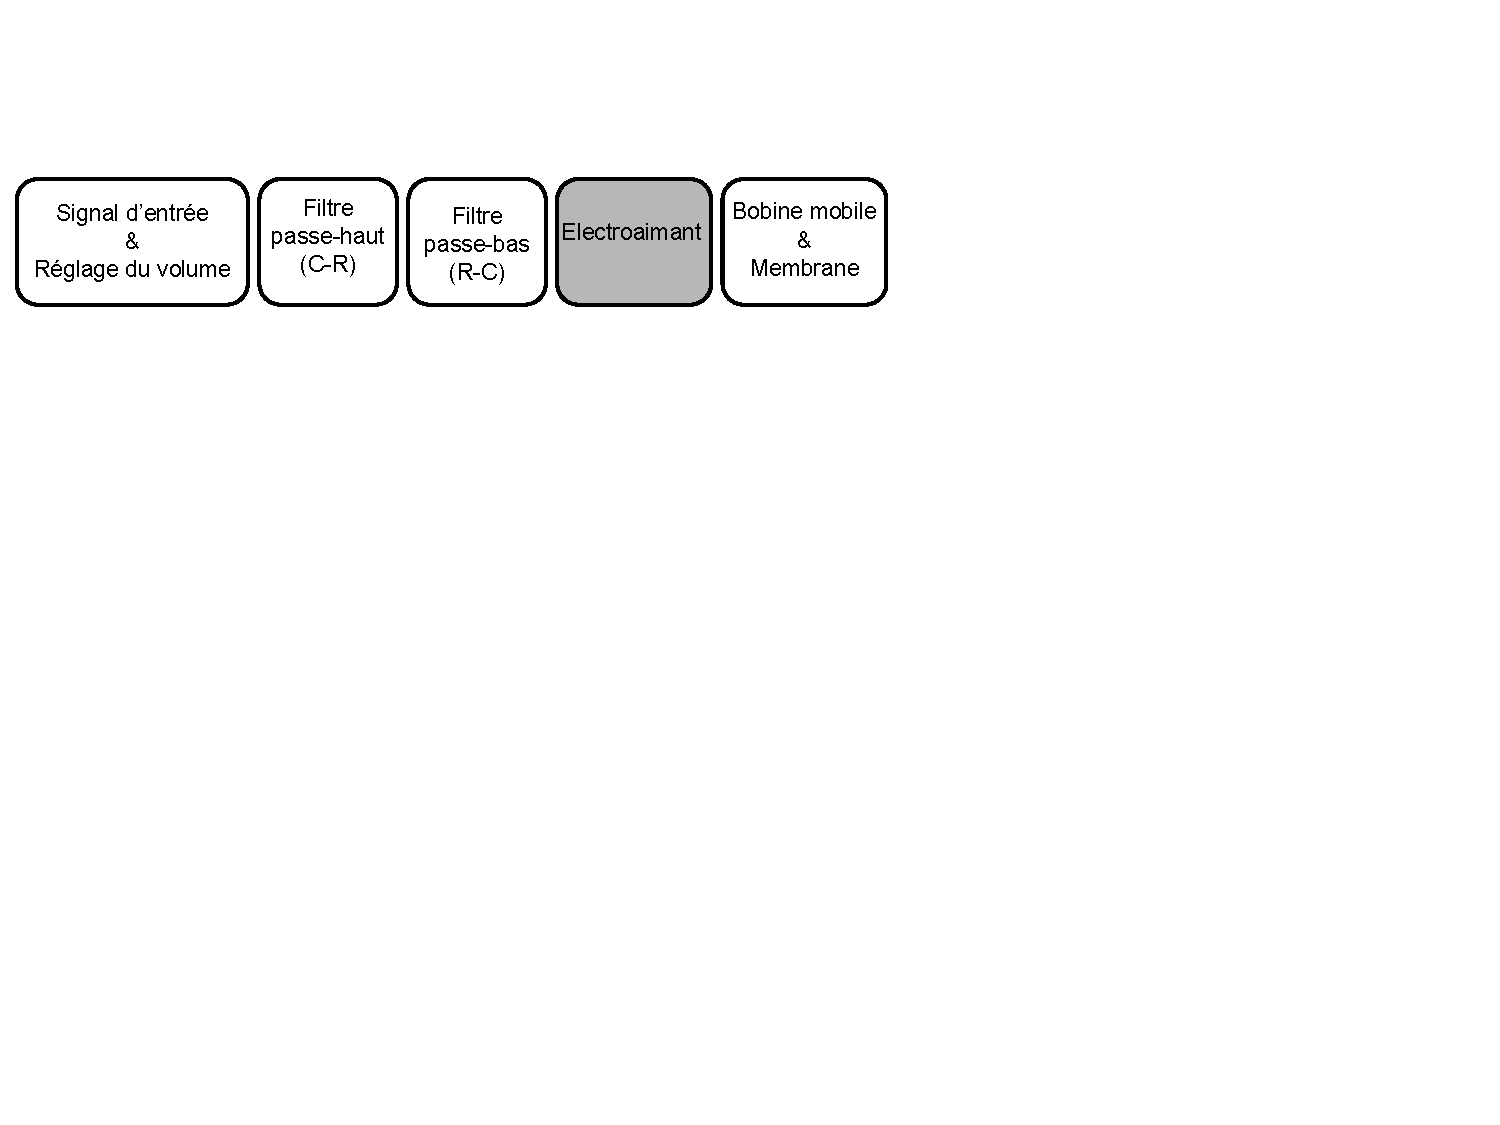
\includegraphics[width=\textwidth]{img/Schemabloc3}
\end{center}

\section{Introduction}
Dans la quasi totalité des haut-parleurs d'aujourd'hui se trouve un aimant permanent générant un champ magnétique.
N'ayant pas de tel aimant à disposition, nous avons réalisé un électro-aimant grâce à du fil de cuivre enroulé autour 
d'un coeur en forme de E de fer doux orienté, matériau ferromagnétique. Ce type de matériau a pour effet d'augmenter très fortement le champ magnétique et d'avoir un cycle d'hystérésis très étroit (donc se démagnétisant rapidement).
\section{Intuition}
Le solénoide étant enroulé sur un coeur magnétique, et l'entrefer étant petit, le champ magnétisant dans 
une boucle passant par le coeur du solénoide, l'entrefer et revenant au solénoide à travers une branche 
du E doit être constant. Ceci pourrait être un bon point de départ pour obtenir le champ $B$ présent dans l'entrefer.

\begin{figure}	
\begin{center}
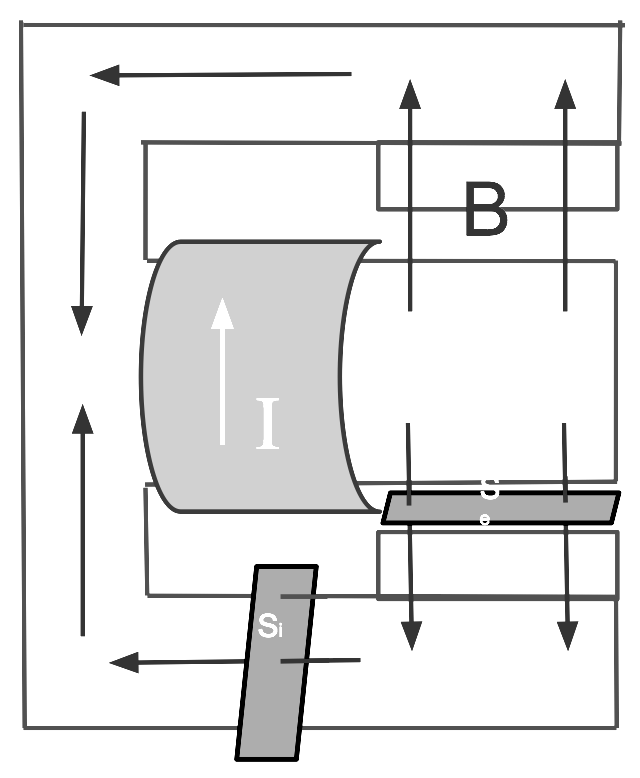
\includegraphics[scale=0.5]{img/schema-aimant-bobine}
\end{center}
\caption{Schema de la bobine fixe}		
\label{fig:bobinefixe}		
\end{figure}

\section{Hypothèses}
\begin{itemize}
\item Le solénoïde étant enroulé autour d'un coeur ferromagnétique ayant $\mu = \mu_0 * 1600$ et puisque les 
tours du solénoïdes sont très fortement serrés, nous supposons qu'aucun champ ne passe entre les fils et que tout le champ magnétique généré passe par l'entrefer.
\item Nous supposons également que tout le champ magnétisant $H$ passe directement par l'entrefer, et que rien ne passe par dessous ou par dessus la branche intermédiaire du E.
\item Le champ $B$ que nous voulons obtenir dans l'entrefer est un champ de $0,1\tesla$. Cette valeur fut choisie car elle nous permet d'obtenir une force suffisante pour faire bouger la membrane avec une amplitude satisfaisante tout en gardant la bobine 
mobile relativement légère en faisant peu de tours de fils de cuivre.
\end{itemize}
Il est à noter que notre entrefer mesure $0.5\centi\meter$ car nous avons rajouté des plaquettes afin de le réduire.

\section{Modélisation}
Le champ magnétisant généré par la bobine est $\int{H dl} = N I$ .
En prenant une boucle dans notre circuit magnétique, grâce à Gauss généralisée, nous avons que
$H_i l + H_e e = N I (1)$
Nous avons également que $B_i S_i = B_e S_e (2)$  avec $S_i \simeq S_e$
ainsi que $B_i = \mu H_i \:et\:  B_e = \mu_0 H_e$
Puisque $\mu \gg \mu_0$ nous savons que $H_i \ll H_e$ grâce à l'équation (2).
Nous pouvons alors réécrire l'équation (1) $H_e = \frac{N I}{e}$.
Nous obtenons alors le champ $B$ recherché $B = B_e = \mu_0 \frac{N I}{e}$.

Puisque nous voulons obtenir un champ $B = 0,1 \tesla$, que nous fournissons $I = 1 A$ afin de ne pas faire trop 
chauffer la bobine, et que nous connaissons $e$, nous pouvons calculer le nombre de tours $N$ requis pour obtenir 0.1\tesla.
$N = \frac{0.1 * 0.5}{\mu_0 * 1} = 400$.

\section{Confrontation}
Grâce à un tesla-mètre, nous avons pu vérifier que notre première hypothèse était correcte, car nous n'obtenions 
qu'environ $10 \milli\tesla$ à côté de la bobine. 

La deuxième hypothèse était cependant trop forte par rapport à la réalité, car une 
partie du champ magnétique passe en dehors de l'entrefer. Afin de palier à ce déficit, nous avons exagéré le nombre de 
tours de la bobine mobile ($N \simeq 550$) et nous avons alors obtenu $B = 112 \milli\tesla$ dans l'entrefer, 
ce qui était le champ désiré (voir l'annexe \ref{mesures champ} p.\pageref{mesures champ}).